\documentclass[11pt]{article}

% ── Packages ──────────────────────────────────────────────────────────────────
\usepackage[utf8]{inputenc}
\usepackage[T1]{fontenc}
\usepackage[spanish,es-noshorthands]{babel}
\usepackage{geometry}
\geometry{a4paper, margin=2.1cm}
\usepackage{amsmath}
\usepackage{graphicx}
\usepackage{booktabs}
\usepackage{hyperref}
\usepackage[table]{xcolor}
\usepackage{tabularx}
\usepackage{enumitem}
\usepackage{titlesec}
\usepackage{fancyhdr}
\usepackage{float}
\usepackage{caption}
\captionsetup{font=footnotesize, labelfont=bf}
\usepackage{tcolorbox}
\tcbuselibrary{skins}

% ── Style ─────────────────────────────────────────────────────────────────────
\hypersetup{colorlinks=true, linkcolor=blue!60!black, urlcolor=blue!70!black, citecolor=blue!60!black}
\setlist{nosep, leftmargin=1.2em}
\titleformat{\section}{\normalfont\sffamily\bfseries\Large\color{black!80}}{\thesection.}{0.5em}{}
\titleformat{\subsection}{\normalfont\sffamily\bfseries\large}{\thesubsection}{0.5em}{}
\titlespacing*{\section}{0pt}{1.6ex plus 0.4ex}{0.8ex plus 0.2ex}
\titlespacing*{\subsection}{0pt}{1.0ex plus 0.3ex}{0.5ex plus 0.1ex}
\pagestyle{fancy}
\fancyhf{}
\fancyhead[L]{\footnotesize\sffamily Resumen Ejecutivo --- Avance 7}
\fancyhead[R]{\footnotesize\sffamily Tecnol\'ogico de Monterrey --- MNA}
\fancyfoot[C]{\thepage}
\renewcommand{\headrulewidth}{0.4pt}
\renewcommand{\footrulewidth}{0pt}

% ── Shortcuts (mismos parches que Conclusions_Avance6.tex, necesarios con babel-spanish) ──
\AtBeginDocument{\def\%{\char37\relax}}
\AtBeginDocument{\renewcommand{\tablename}{Tabla}\addto\captionsspanish{\renewcommand{\tablename}{Tabla}}}
\newcommand{\ghref}[2]{\href{https://github.com/alejandrogonzalz/trading_management/blob/dev/#1}{#2}}

% ── Colores de marca ──────────────────────────────────────────────────────────
\definecolor{brandteal}{RGB}{0,121,107}
\definecolor{brandblue}{RGB}{30,76,124}
\definecolor{brandamber}{RGB}{183,121,0}
\definecolor{brandred}{RGB}{158,42,43}
\definecolor{brandpurple}{RGB}{93,64,140}
\definecolor{brandgray}{RGB}{245,245,245}

% ── Tarjeta KPI ───────────────────────────────────────────────────────────────
\newtcolorbox{kpi}[1]{
  colback=#1!6, colframe=#1!55!black, boxrule=0.7pt, arc=1.5mm,
  width=\linewidth, height=3.55cm, valign=center, halign=center,
  boxsep=2pt, left=2pt, right=2pt
}
\newcommand{\kpicard}[4]{%
  \begin{minipage}{0.235\linewidth}
    \begin{kpi}{#4}
      {\fontsize{19}{21}\selectfont\sffamily\bfseries\color{#4!60!black} #1}\\[0.45em]
      {\footnotesize\sffamily #2}\\[0.15em]
      {\scriptsize\itshape\color{black!55} #3}
    \end{kpi}
  \end{minipage}
}

% ── Panel de riesgo (caja tem\'atica con color por categor\'ia) ───────────────
\newtcolorbox{riskpanel}[2]{
  colback=#2!5, colframe=#2!55!black, boxrule=0.8pt, arc=1.5mm,
  width=\linewidth, valign=top, title={\sffamily\bfseries #1},
  fonttitle=\sffamily\bfseries\color{white}, colbacktitle=#2!55!black,
  boxsep=3pt, left=4pt, right=4pt, top=2pt, bottom=2pt
}

% ── Caja de decisi\'on / TL;DR ────────────────────────────────────────────────
\newtcolorbox{calloutbox}[2]{
  colback=#2!7, colframe=#2!60!black, boxrule=1pt, arc=1.5mm,
  width=\linewidth, title={\sffamily\bfseries #1},
  fonttitle=\sffamily\bfseries\color{white}, colbacktitle=#2!60!black,
  boxsep=4pt, left=6pt, right=6pt
}

% ══════════════════════════════════════════════════════════════════════════════
\begin{document}
\thispagestyle{empty}

% ── Portada ejecutiva ─────────────────────────────────────────────────────────
\begin{center}

\includegraphics[height=1.6cm]{figures/executive_summary/logo_itesm.png}\\[1.1em]
{\sffamily\bfseries\LARGE Resumen Ejecutivo\par}
\vspace{0.4em}
{\sffamily\Large De la investigaci\'on al producto: un LLM ajustado como n\'ucleo de decisi\'on para trading de criptomonedas\par}
\vspace{0.9em}
{\small Alejandro Gonz\'alez Almaz\'an\textsuperscript{1} \quad Dra. Alicia Fernanda Galindo Manrique\textsuperscript{1}\\[0.2em]
\textsuperscript{1}Tecnol\'ogico de Monterrey --- Maestr\'ia en Inteligencia Artificial Aplicada\\[0.2em]
\textit{Avance 7 --- Junio 2026}\par}
\end{center}

\vspace{0.6em}
\begin{calloutbox}{S\'intesis ejecutiva}{brandteal}
El presente proyecto especializ\'o, mediante \textit{fine-tuning} (QLoRA), un modelo de lenguaje de 7\,mil millones de par\'ametros perteneciente a la misma familia (Qwen~2.5) que opera actualmente en el sistema. El modelo final se entren\'o en una sola corrida de 3.6\,h ($\sim$\$5 USD de GPU en la nube), y todo el ciclo de investigaci\'on ---incluidas las corridas de ablaci\'on y robustez--- se mantuvo por debajo de \$20 USD. Con esa inversi\'on de c\'omputo, el modelo pas\'o de un desempe\~no que destruye capital en simulaci\'on (\textit{profit factor} de 0.70) a uno situado en el rango profesional de los sistemas de \textit{trading} (\textit{profit factor} de 2.09 y 84.13\,\% de exactitud direccional). La hip\'otesis central del proyecto ---que la especializaci\'on de dominio supera al modelo gen\'erico--- se confirma con una mejora estad\'isticamente significativa ($\chi^2=1{,}949$, $p\approx0$), tanto respecto de la versi\'on sin ajustar como de cualquier modelo cl\'asico de \textit{Machine Learning} evaluado.
\end{calloutbox}

\vspace{0.8em}
\noindent
\kpicard{84.13\,\%}{Exactitud direccional}{Modelo final, sin sesgo de supervivencia (validaci\'on McNemar, $p\approx0$)}{brandteal}\hfill
\kpicard{PF 2.09}{Factor de ganancia}{Simulaci\'on sin circularidad (ATR) --- rango profesional (Pardo, 2008)}{brandblue}\hfill
\kpicard{$\sim$\$5}{Costo del modelo final}{1 corrida QLoRA, 3.6\,h en A100 80GB (\$1.42/h); todo el I+D $<$\$20}{brandamber}\hfill
\kpicard{\$0.02 / 1k}{Costo por predicci\'on}{Ollama local; o Together AI gestionado, sin operar GPU propia}{brandpurple}

\vspace{1em}
\noindent\textbf{Qu\'e se le pide al lector de este documento:} aprobar un periodo de 4 semanas de \textit{paper trading} (sin capital real) y un presupuesto operativo estimado de \$15--25 USD/mes, como condici\'on previa --- ya identificada por el propio equipo --- antes de considerar capital real (ver \S7).

\vspace{0.6em}
\hrule
\vspace{1.2em}

% ── 1. S\'intesis del problema ─────────────────────────────────────────────────
\section{S\'intesis del problema}

Los mercados de criptomonedas son dif\'iciles de predecir: la relaci\'on se\~nal-ruido es baja y los reg\'imenes de mercado cambian sin aviso. Los modelos de Machine Learning cl\'asico que la industria usa hoy ---\'arboles de decisi\'on, redes recurrentes--- tocan un techo conocido de alrededor del 60--65\,\% de exactitud direccional, sin importar cu\'anto se optimicen sus hiperpar\'ametros. Por otro lado, los modelos de lenguaje de gran escala (LLMs) prometen algo distinto: pueden razonar sobre indicadores t\'ecnicos en lenguaje natural, tal como lo har\'ia un analista humano, y producir no solo una etiqueta sino una decisi\'on estructurada (entrada, toma de ganancia, p\'erdida l\'imite, justificaci\'on). El riesgo es que, sin especializaci\'on de dominio, esa promesa se queda en papel: el mismo LLM en modo \textit{zero-shot} ---es decir, sin haber visto un solo ejemplo de nuestra tarea--- alcanza apenas 56.5\,\% de exactitud y, lo m\'as importante para un negocio, \textbf{pierde capital de forma sostenida} en simulaci\'on (\textit{profit factor} de 0.70: por cada \$1 perdido, recupera solo \$0.70).

La oportunidad es concreta: especializar ese mismo modelo en nuestra tarea espec\'ifica mediante \textit{fine-tuning} con adaptadores de bajo rango (QLoRA), sin entrenar un modelo desde cero ni adquirir infraestructura nueva, y medir si el resultado es lo bastante s\'olido para servir como n\'ucleo de decisi\'on de un agente de \textit{trading} aut\'onomo que ya est\'a en desarrollo (arquitectura LangGraph, descrita en el Avance 6). La \textbf{hip\'otesis} que articula el proyecto es directa: un modelo de lenguaje especializado en el dominio superar\'a, por un margen sustancial, tanto al mismo modelo gen\'erico (\textit{zero-shot}) como a los modelos cl\'asicos de Machine Learning, en exactitud direccional y en viabilidad operativa.

La Figura~\ref{fig:exec-pipeline} ilustra c\'omo opera hoy el sistema en producci\'on: un \textit{scanner} cuantitativo calcula un \textit{Quant Score} multifactor sobre m\'as de 20 pares y 7 \textit{timeframes}, y los candidatos resultantes se env\'ian a Qwen~2.5~14B en modo \textit{zero-shot} ---v\'ia Ollama--- para que identifique y razone sobre los mejores \textit{setups}. Ese nodo es precisamente el componente que este proyecto somete a evaluaci\'on: como ya se documenta en esta secci\'on, sin especializaci\'on de dominio el modelo pierde capital de forma sostenida.

\begin{figure}[H]
\centering
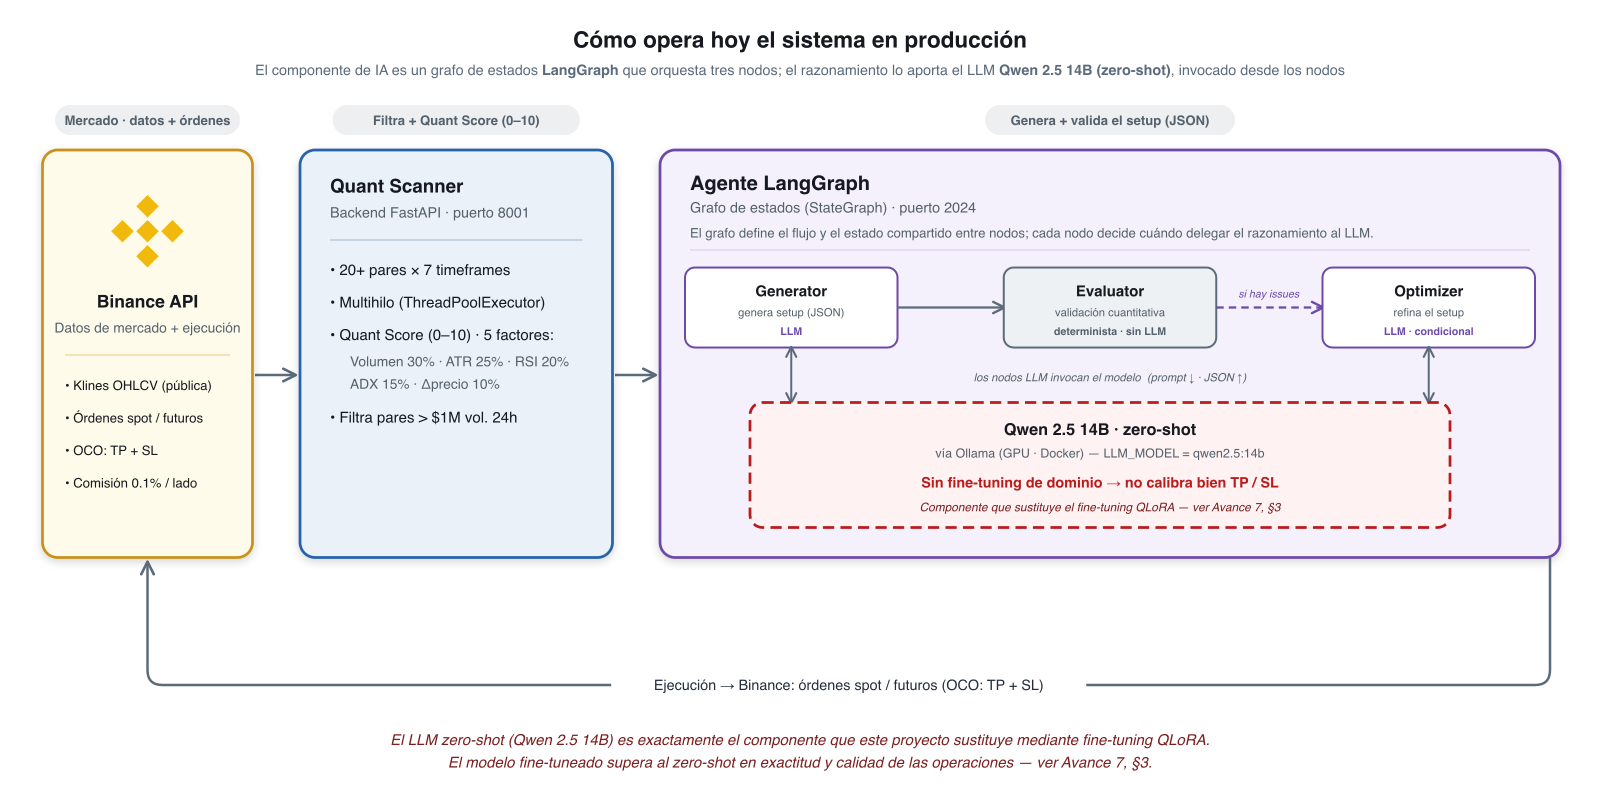
\includegraphics[width=\linewidth]{figures/executive_summary/fig_production_pipeline.png}
\caption{Arquitectura de producci\'on actual. El \textit{scanner} cuantitativo alimenta de indicadores t\'ecnicos al LLM, que opera en modo \textit{zero-shot} dentro del agente LangGraph ---un grafo de estados de tres nodos: generaci\'on (LLM) $\rightarrow$ validaci\'on cuantitativa determinista $\rightarrow$ optimizaci\'on condicional (LLM)--- antes de ejecutar la orden en Binance. El nodo flageado (el LLM \textit{zero-shot}) es el que este trabajo sustituye mediante \textit{fine-tuning}. El sistema en producci\'on usa la variante 14B; la l\'inea base \textit{zero-shot} y el modelo ajustado se midieron sobre la variante 7B del mismo modelo, para que la comparaci\'on aisle el efecto de la especializaci\'on y no el del tama\~no (\S3).}
\label{fig:exec-pipeline}
\end{figure}

Que ese nodo est\'e envuelto en un grafo de estados ---y no invocado de forma aislada--- no es incidental. El agente, implementado sobre LangGraph, es un grafo dirigido de tres nodos con una arista condicional: \textit{generator} (el LLM propone un \textit{setup}), \textit{evaluator} (validaci\'on cuantitativa \textbf{determinista}, sin LLM: verifica coherencia de entrada/TP/SL, RSI, ATR, riesgo de liquidaci\'on y confluencia multi-\textit{timeframe}) y, solo si el evaluador detecta problemas, \textit{optimizer} (el LLM refina la propuesta). El LLM, por tanto, se invoca \'unicamente dentro de los nodos \textit{generator} y \textit{optimizer}; \textbf{es exactamente ese componente de razonamiento el que este proyecto sustituye mediante \textit{fine-tuning}}, mientras que el nodo \textit{evaluator} es l\'ogica determinista que no se ve afectada por el ajuste. Este dise\~no ---razonar, validar con reglas duras y solo entonces refinar--- toma inspiraci\'on del paradigma \textbf{ReAct} (\textit{Reasoning and Acting}; Yao et al., 2023), que entrelaza razonamiento y acci\'on en un bucle Pensamiento $\rightarrow$ Acci\'on $\rightarrow$ Observaci\'on; la evoluci\'on natural del agente hacia un bucle ReAct completo, con uso aut\'onomo de herramientas, es trabajo futuro (\S6). La literatura reciente respalda la apuesta por invertir en la arquitectura del agente: en el \textit{benchmark} \textit{Agent Market Arena}, un agente ReAct sobre GPT-4.1 alcanz\'o un \textit{Sharpe ratio} de 6.47 en TSLA, y los autores concluyen que la arquitectura del agente pesa m\'as que la capacidad del modelo subyacente (Qian et al., 2026); en \textit{Auto Trader X}, un \textit{framework} ag\'entico con RAG alcanz\'o 68.4\,\% de exactitud direccional ---frente a 52.3\,\% de ARIMA y 57.1\,\% de LSTM--- con un \textit{Sharpe ratio} de 2.10, un \textit{drawdown} m\'aximo de $-$11.2\,\% y una latencia de 780\,ms, viable para \textit{trading} institucional (Swayam et al., 2026). Lo que este proyecto aporta es especializar el componente de razonamiento que opera dentro de esa arquitectura.

Este documento resume la evidencia de los Avances 0--6 y la organiza en torno a tres preguntas que cualquier tomador de decisiones se plantea ante una propuesta de IA: \textbf{?`funciona mejor que las alternativas?} (\S2--\S3), \textbf{?`cu\'anto cuesta construirlo y operarlo?} (\S5) y \textbf{?`qu\'e puede salir mal?} (\S6). Las secciones siguientes responden cada una en ese orden, cerrando con una recomendaci\'on accionable y acotada (\S7).

% ── 2. Hallazgos del EDA ───────────────────────────────────────────────────────
\section{Hallazgos m\'as importantes del an\'alisis exploratorio de datos}

La base de evidencia de este proyecto (Avance 1, An\'alisis Exploratorio de Datos) se construy\'o descargando hist\'orico real de Binance para 12 criptomonedas durante 18 meses (diciembre 2023 -- junio 2025), calculando indicadores t\'ecnicos est\'andar (RSI, MACD, ADX, ATR, Bandas de Bollinger, entre otros) en tres resoluciones temporales (1h, 4h, 1d), y etiquetando cada punto de decisi\'on seg\'un lo que efectivamente ocurri\'o despu\'es. Cuatro hallazgos de esa etapa son relevantes para la decisi\'on de negocio:

\begin{itemize}
\item \textbf{Calidad sobre cantidad}: de $\sim$250{,}000 velas crudas, solo el 22.4\,\% super\'o los filtros de calidad (volumen, fuerza de tendencia, relaci\'on riesgo-recompensa, ausencia de reversi\'on temprana), produciendo 56{,}161 muestras de alto valor predictivo. El modelo final, adem\'as, se valid\'o tambi\'en sobre las 75{,}289 muestras \emph{sin} ese filtro, para no maquillar el resultado (\S3).
\item \textbf{Sin sesgo de clase}: el balance LONG/SHORT es casi perfecto (49\,\% / 51\,\%), por lo que la exactitud reportada no es un efecto de "adivinar siempre lo mismo".
\item \textbf{Diversidad de activos}: la muestra cubre tres perfiles de capitalizaci\'on y volatilidad (BTC/ETH/BNB, SOL/XRP/ADA/AVAX/DOT, DOGE/LINK/MATIC/NEAR) --- la evidencia no depende de un solo activo.
\item \textbf{Gobernanza de datos desde el dise\~no}: la partici\'on en entrenamiento/validaci\'on/prueba es estrictamente cronol\'ogica, con una "zona de seguridad" (\textit{embargo}) de 24 horas en cada frontera para garantizar que ninguna muestra de prueba se haya visto, ni parcialmente, durante el entrenamiento. Esto es relevante para el lector de negocio porque es precisamente el tipo de error ---fuga de informaci\'on futura--- que infla artificialmente resultados de IA financiera y que aqu\'i se dise\~n\'o para evitar desde el inicio.
\end{itemize}

\begin{figure}[H]
\centering

\includegraphics[width=0.85\linewidth]{figures/executive_summary/fig_temporal_split.png}
\caption{Partici\'on temporal con embargo de 24h en cada frontera: entrenamiento (m\'as antiguo) $\rightarrow$ validaci\'on $\rightarrow$ prueba (m\'as reciente). Ninguna muestra de prueba pudo haber sido vista, ni parcialmente, durante el entrenamiento.}
\label{fig:exec-split}
\end{figure}

\noindent Con datos limpios y una evaluaci\'on a prueba de fugas, la siguiente pregunta es la de fondo: sobre esa misma base, ?`qu\'e enfoque predice mejor y, sobre todo, opera de forma rentable?

% ── 3. Modelos generados y elecci\'on del modelo final ─────────────────────────
\section{Modelos generados y razones de la elecci\'on del modelo final}

El Avance 5 compar\'o cinco familias de modelos sobre exactamente el mismo conjunto de prueba: \'arboles de decisi\'on (XGBoost, Random Forest), una red recurrente (LSTM), el LLM gen\'erico sin ajustar (\textit{zero-shot}) y el mismo LLM especializado mediante \textit{fine-tuning} (QLoRA). La Tabla~\ref{tab:exec-comparativa} resume el resultado. Todas las m\'etricas financieras se calculan con la simulaci\'on \textit{forward-looking} basada en ATR ---que fija los niveles de salida con informaci\'on disponible al momento de la decisi\'on, no en retrospectiva--- por lo que no contienen la circularidad que infla artificialmente este tipo de resultados.

\begin{table}[H]
\centering
\caption{Comparativa de enfoques sobre el mismo conjunto de prueba (simulaci\'on financiera ATR, sin circularidad)}
\label{tab:exec-comparativa}
\small
\begin{tabularx}{\linewidth}{Xccc}
\toprule
\textbf{Enfoque} & \textbf{Exactitud} & \textbf{Win rate} & \textbf{Profit factor} \\
\midrule
\textbf{LLM ajustado (QLoRA, modelo final)} & \textbf{84.13\,\%} & \textbf{66.3\,\%} & \textbf{2.09} \\
XGBoost (mejor modelo ML cl\'asico) & 62.7\,\% & 57.5\,\% & 1.53 \\
LLM sin ajustar (\textit{zero-shot}) & 56.49\,\% & 39.9\,\% & 0.70 \\
LSTM & 51.51\,\% & 46.7\,\% & 1.49 \\
\bottomrule
\end{tabularx}
{\scriptsize El \textit{profit factor} de 1.5--2.5 corresponde al rango de sistemas de \textit{trading} profesionalmente viables (Pardo, 2008); por debajo de 1.0 el sistema destruye capital. La Figura~\ref{fig:exec-beforeafter} contrasta visualmente el antes/despu\'es del ajuste.}
\end{table}

\begin{figure}[H]
\centering
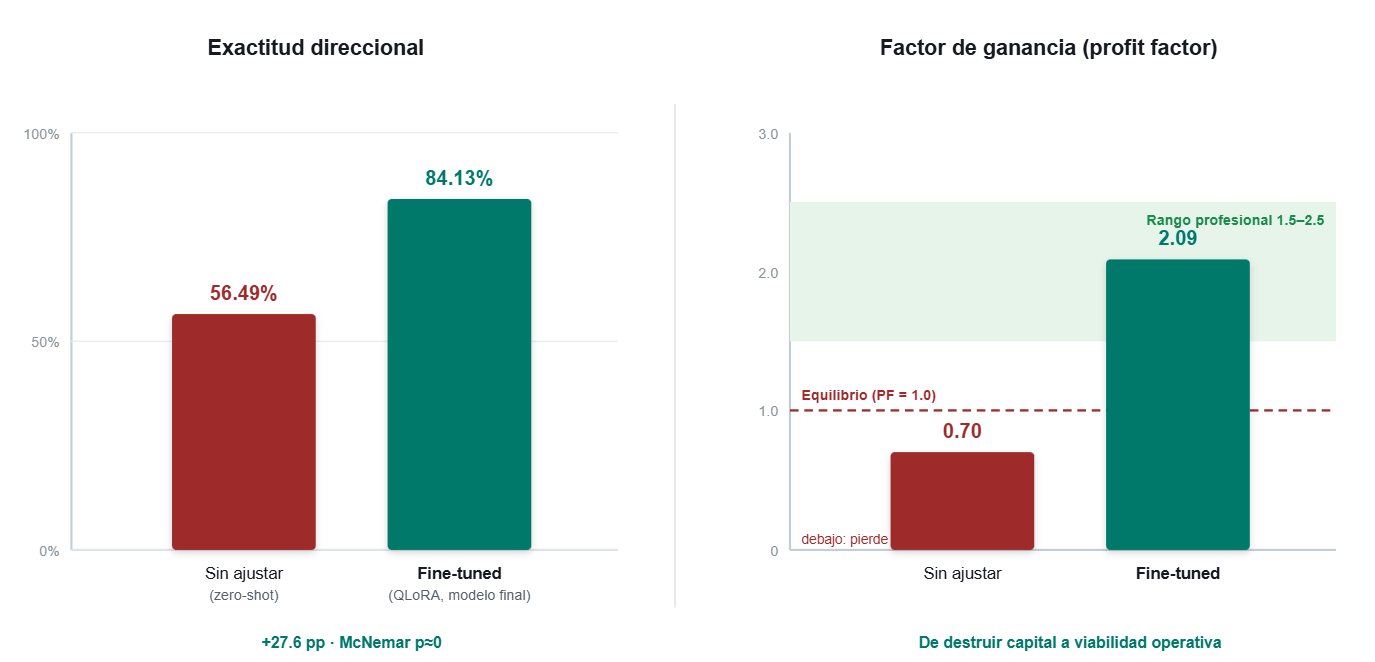
\includegraphics[width=\linewidth]{figures/executive_summary/fig_before_after.png}
\caption{El efecto del \textit{fine-tuning} sobre el mismo modelo base. Izquierda: la exactitud direccional sube de 56.49\,\% a 84.13\,\% ($+$27.6\,pp). Derecha: el \textit{profit factor} cruza de 0.70 (destruye capital) a 2.09 (rango profesional). No es una mejora marginal: cambia la viabilidad operativa del sistema.}
\label{fig:exec-beforeafter}
\end{figure}

\begin{figure}[H]
\centering
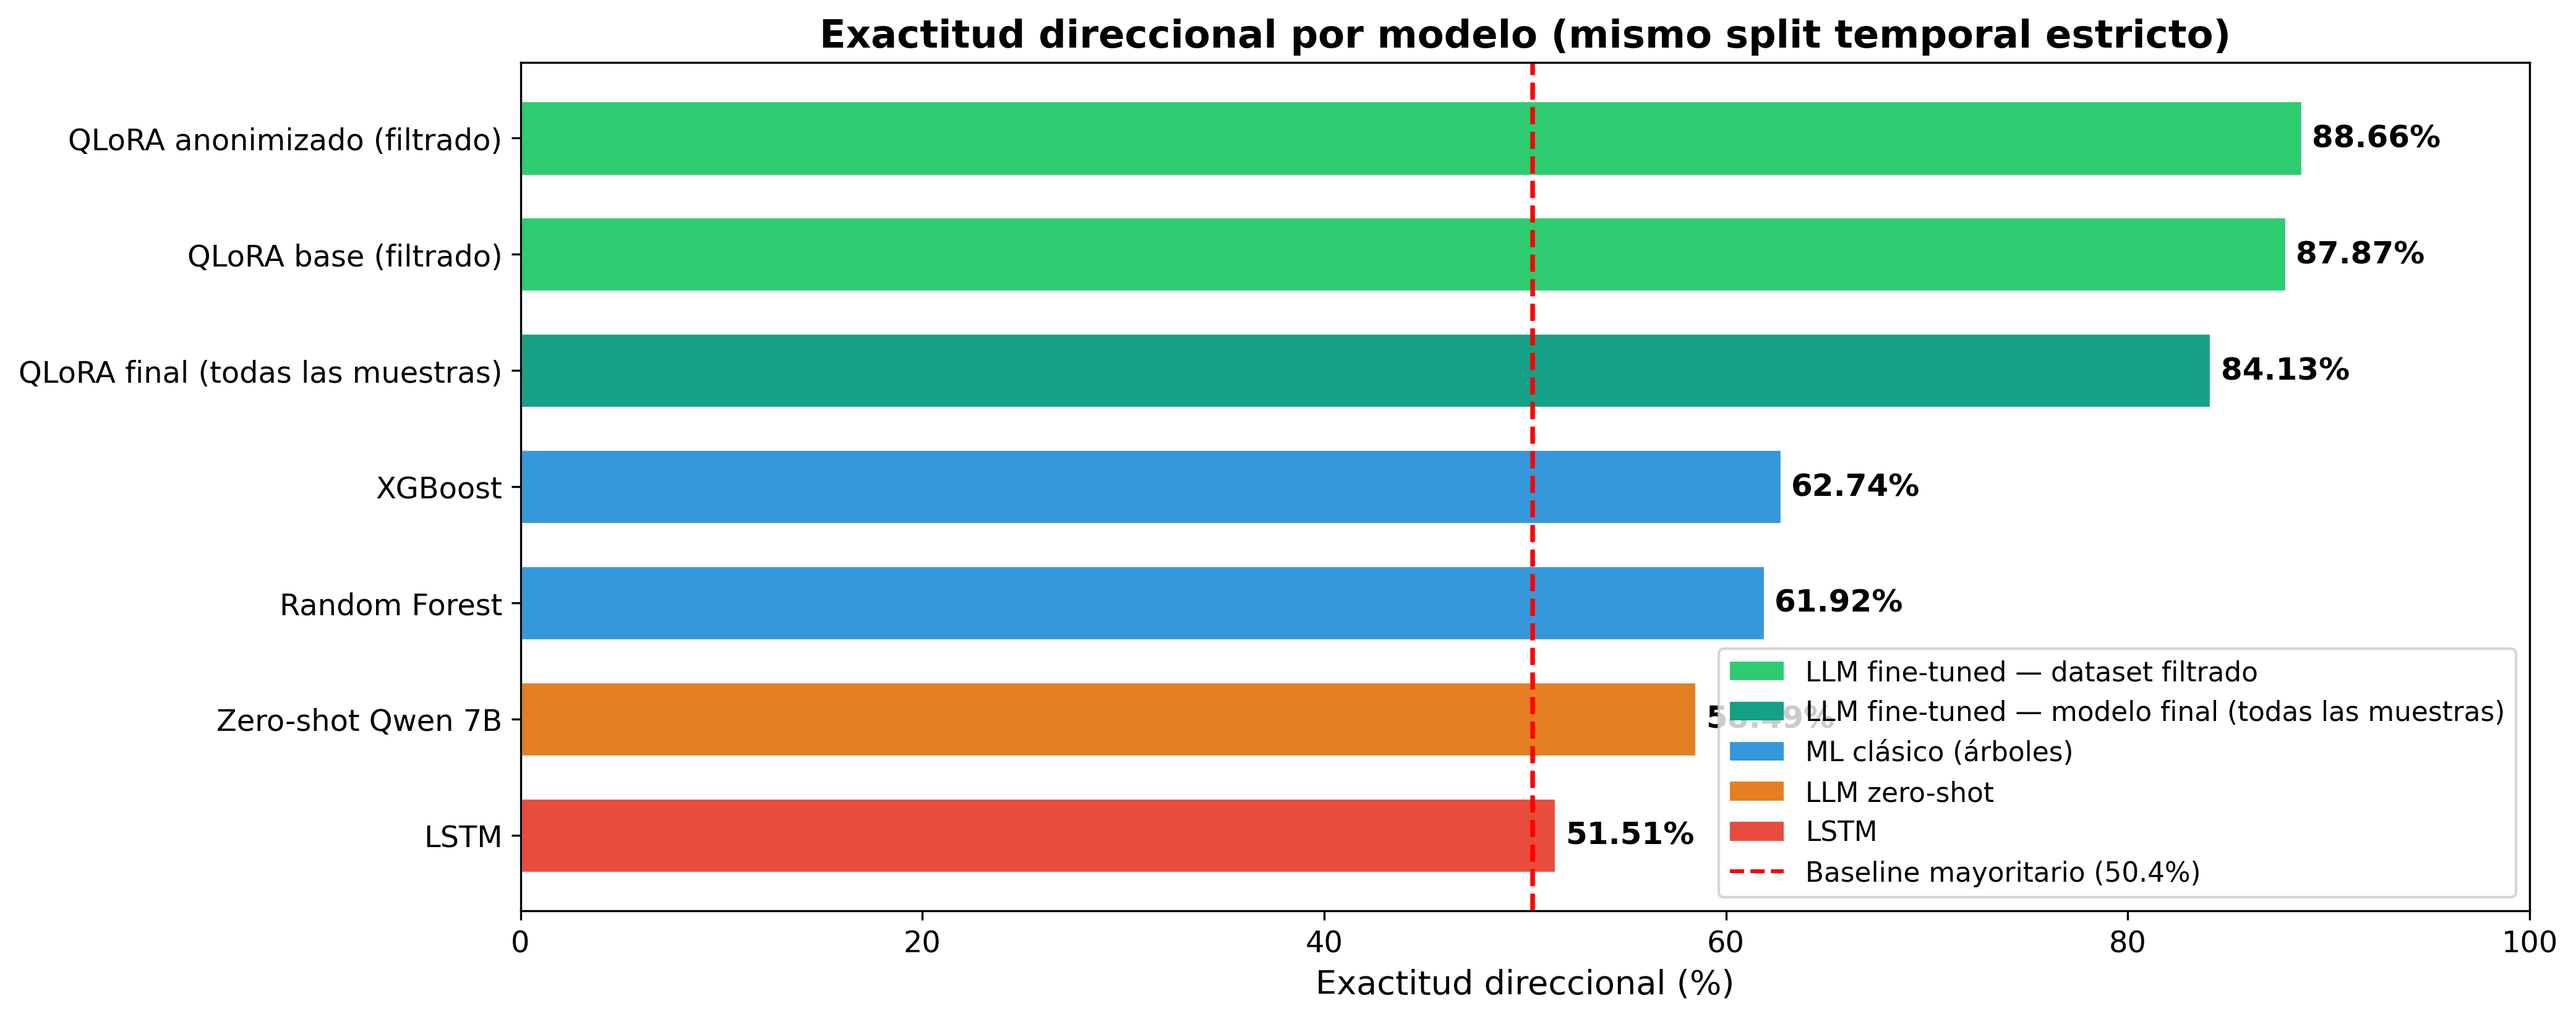
\includegraphics[width=0.92\linewidth]{figures/executive_summary/fig4_accuracy_all_models.png}
\caption{Exactitud direccional por modelo sobre el mismo conjunto de prueba. Los modelos cl\'asicos ---\'arboles y LSTM--- se agrupan cerca o por debajo del 64\,\%; las variantes del modelo ajustado los superan por m\'as de 20 puntos porcentuales, y a la l\'inea base \textit{zero-shot} por m\'as de 25.}
\label{fig:exec-accuracy}
\end{figure}

Tres conclusiones explican por qu\'e el modelo ajustado es la recomendaci\'on, y no simplemente "el de mayor n\'umero":

\begin{enumerate}
\item \textbf{No es un techo de esfuerzo, es un techo de representaci\'on.} Los modelos de \'arbol se optimizaron exhaustivamente (150 combinaciones de hiperpar\'ametros para XGBoost, 80 para Random Forest) y aun as\'i no superan $\sim$64\,\%. El l\'imite no es cu\'anto buscamos, sino que estos modelos solo ven n\'umeros sueltos, mientras que el LLM lee los mismos indicadores en el formato textual que un analista usar\'ia.
\item \textbf{El conocimiento gen\'erico no basta; la especializaci\'on de dominio s\'i.} El mismo modelo base, sin ajuste, "sabe" parcialmente (56.5\,\%) pero no sabe operar: pierde dinero. El \textit{fine-tuning} es la diferencia entre un modelo inviable y uno rentable --- y esa diferencia es estad\'isticamente inequ\'ivoca (prueba de McNemar, $\chi^2=1{,}949$, $p\approx0$, sobre 11{,}294 decisiones pareadas).
\item \textbf{Elegimos el resultado conservador, no el m\'as alto.} Existe una variante del modelo que alcanza 88.66\,\% de exactitud (\textit{profit factor} 4.63), pero se entrena y eval\'ua sobre el subconjunto de \textit{setups} ya filtrados como "limpios": su cifra es optimista y su \textit{profit factor} ---por encima de 4--- entra en el territorio que la propia literatura considera sospechoso de sobreajuste. El \textbf{modelo final recomendado} (84.13\,\%, \textit{profit factor} 2.09) se entrena sobre \emph{todas} las muestras disponibles, sin ese filtro, y es por tanto el n\'umero m\'as defendible frente a condiciones de mercado reales. Adem\'as, generaliza de forma pareja: entre los 11 activos evaluados individualmente la exactitud var\'ia apenas 4.6 puntos porcentuales (81.8\,\%--86.4\,\%) --- no depende de "acertarle" a una sola criptomoneda.
\end{enumerate}

Por transparencia metodol\'ogica conviene precisar una decisi\'on de dise\~no: el sistema en producci\'on usa Qwen~2.5 \textbf{14B}, pero el \textit{fine-tuning} se hizo sobre la versi\'on \textbf{7B} del mismo modelo, y el \textit{zero-shot} se midi\'o tambi\'en sobre 7B. Esto es deliberado: comparar 7B-ajustado contra 7B-sin-ajustar a\'isla el efecto de la \textit{especializaci\'on} del efecto del \textit{tama\~no}, de modo que la ventaja observada se atribuya inequ\'ivocamente al ajuste de dominio y no a un modelo m\'as grande.

\begin{tcolorbox}[colback=black!3, colframe=black!45, boxrule=0.7pt, arc=1.5mm, title={\sffamily\bfseries Ficha t\'ecnica del modelo (para stakeholders t\'ecnicos)}, fonttitle=\sffamily\bfseries\color{white}, colbacktitle=black!55, boxsep=3pt, left=5pt, right=5pt]
\footnotesize
\begin{tabularx}{\linewidth}{lX}
Modelo base & Qwen~2.5~7B~Instruct, cuantizado a 4 bits (NF4) \\
T\'ecnica & QLoRA --- adaptadores de bajo rango (\textit{rank}=16, $\alpha$=32) \\
Par\'ametros entrenables & 40.4 M = 0.53\,\% del total (el modelo base permanece congelado) \\
Longitud de secuencia & 1{,}024 \textit{tokens} \\
Infraestructura & GPU NVIDIA A100 80GB (nube); \textit{early stopping} en 2 \'epocas \\
Partici\'on & Temporal estricta 70/15/15 + embargo de 24h (sin fuga) \\
Evaluaci\'on & Conjunto de prueba completo (11{,}294 muestras), IC\,95\,\% $\approx\pm$0.7\,pp \\
Validaci\'on estad\'istica & McNemar pareada vs.\ \textit{zero-shot}: $\chi^2=1{,}949$, $p\approx0$ \\
\end{tabularx}
\end{tcolorbox}

En resumen, la respuesta a la primera pregunta de negocio es afirmativa y robusta: el modelo ajustado predice mejor y, a diferencia del \textit{zero-shot}, opera de forma rentable. La siguiente pregunta es c\'omo llevarlo a producci\'on.

% ── 4. Recomendaciones clave de implementaci\'on ───────────────────────────────
\section{Recomendaciones clave para implementar la soluci\'on}

El Avance 6 tradujo estos resultados en una hoja de ruta de tres fases, ya secuenciada por urgencia y dependencias t\'ecnicas:

\begin{description}
\item[Fase 1 --- Activaci\'on (sin bloqueadores t\'ecnicos).] El modelo ajustado ya existe como artefacto entrenado. El paso restante es t\'ecnico y r\'apido: servirlo v\'ia Together AI (API gestionada) u Ollama en un servidor propio, y conectarlo como n\'ucleo de razonamiento del agente LangGraph que ya opera en producci\'on con el modelo gen\'erico. No requiere nueva infraestructura de entrenamiento.
\item[Fase 2 --- Validaci\'on en vivo sin riesgo (4 semanas).] Antes de comprometer capital real, el propio equipo defini\'o como condici\'on obligatoria un periodo de \textit{paper trading} (operaci\'on simulada sobre datos de mercado en vivo) con monitoreo continuo de exactitud. Esto cierra la brecha entre "funciona en backtest hist\'orico" y "funciona en condiciones actuales de mercado".
\item[Fase 3 --- Maduraci\'on (no bloqueante para activar la Fase 1).] L\'ineas de mejora continua: calibrar la confianza del modelo para dimensionar posiciones proporcionalmente al riesgo, validar con m\'ultiples ventanas de tiempo (\textit{walk-forward}), reentrenar peri\'odicamente ante el desgaste del modelo (\textit{drift}) ---la mitigaci\'on directa del riesgo de cambio de r\'egimen de \S6--- y poner a prueba el sistema en un mercado bajista, dado que el periodo evaluado fue predominantemente alcista.
\end{description}

\begin{figure}[H]
\centering
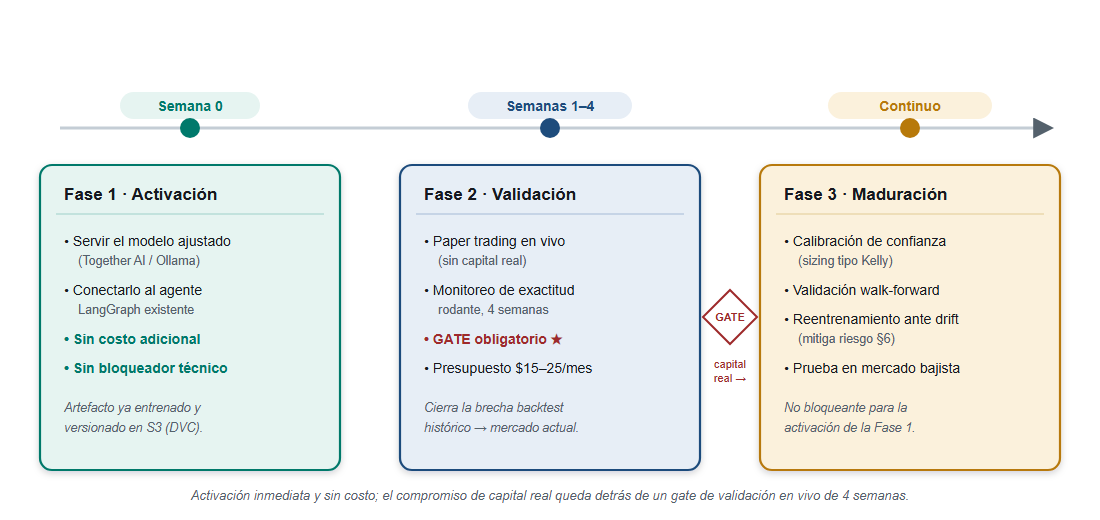
\includegraphics[width=\linewidth]{figures/executive_summary/fig_roadmap.png}
\caption{Hoja de ruta de despliegue en tres fases. La activaci\'on (Fase 1) es inmediata y sin costo; el compromiso de capital real queda condicionado a superar un \textit{gate} de validaci\'on en vivo (Fase 2). La maduraci\'on (Fase 3) corre en paralelo sin bloquear las anteriores.}
\label{fig:exec-roadmap}
\end{figure}

La arquitectura de despliegue propuesta (Figura~\ref{fig:exec-lightsail}) separa deliberadamente el servidor de aplicaci\'on (sin GPU, bajo costo) de la inferencia del modelo, de modo que cada componente escale de forma independiente y el costo de mantener el sistema corriendo permanezca bajo. La elecci\'on de \textbf{AWS Lightsail} en particular ---y no una alternativa \textit{serverless}--- no es incidental: Lightsail asigna una \textbf{direcci\'on IP p\'ublica est\'atica} al servidor de aplicaci\'on, y Binance exige restringir cada llave de API a una IP fija por motivos de seguridad. Un entorno \textit{serverless} (IP ef\'imera, distinta en cada invocaci\'on) no cumple ese requisito sin una capa adicional de red. La inferencia del modelo, por su parte, se delega a \textbf{Together AI} (API gestionada, sin operar GPU propia) o a un servidor con \textbf{Ollama} si se prefiere mantener el modelo en infraestructura propia --- en ambos casos, fuera del servidor de aplicaci\'on, para que escale de forma independiente.

\begin{figure}[H]
\centering
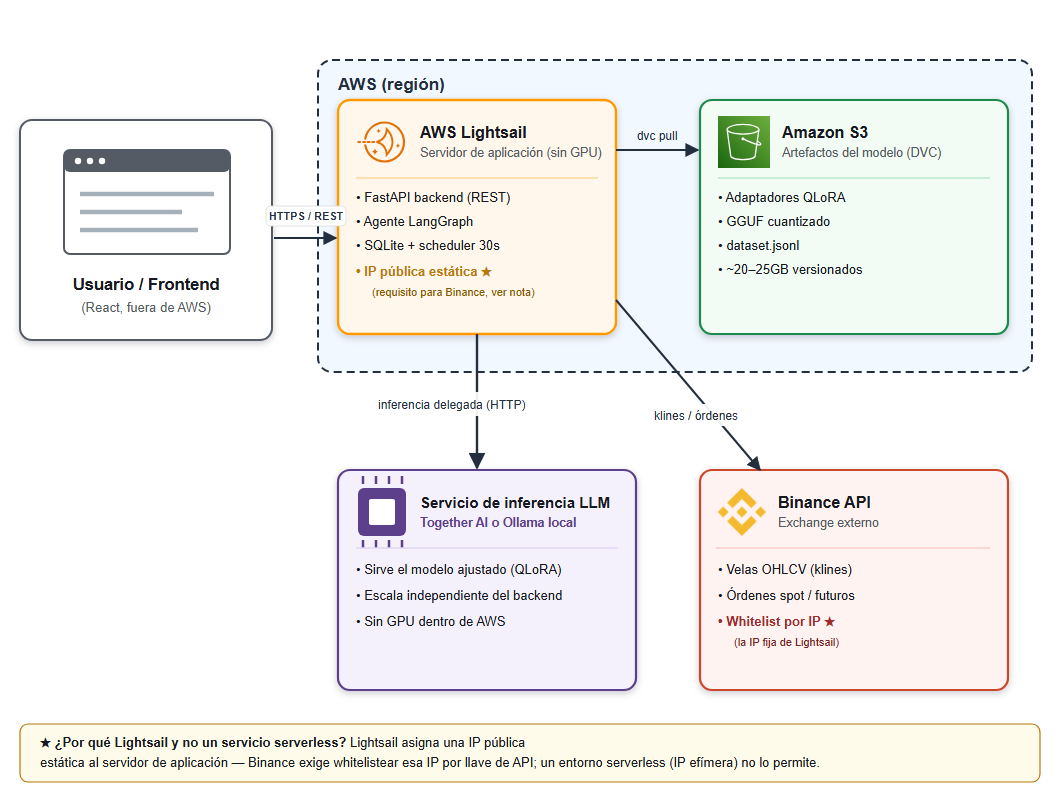
\includegraphics[width=0.95\linewidth]{figures/executive_summary/fig_lightsail_aws.png}
\caption{Arquitectura de despliegue propuesta sobre AWS: el servidor de aplicaci\'on (AWS Lightsail) no requiere GPU y aporta la IP p\'ublica est\'atica que Binance exige para autorizar la llave de API; la inferencia se delega a un servicio especializado (Together AI u Ollama local), y los artefactos del modelo se versionan en Amazon S3. Cada componente escala de forma independiente.}
\label{fig:exec-lightsail}
\end{figure}

\noindent Establecida la viabilidad t\'ecnica y la ruta de despliegue, la decisi\'on pasa por la econom\'ia del proyecto: qu\'e cost\'o llegar hasta aqu\'i, qu\'e costar\'a operarlo y qu\'e beneficios concretos entrega.

% ── 5. An\'alisis costo -- beneficio ────────────────────────────────────────────
\section{An\'alisis costo -- beneficio}
\label{sec:costos}

\subsection{Costos incurridos a la fecha, por fase de la metodolog\'ia CRISP-ML}

La Tabla~\ref{tab:costos-fase} desglosa todo el costo de c\'omputo del proyecto hasta hoy, fase por fase. El supuesto rector es conservador: solo se cuentan cargos reales de proveedores externos (GPU en la nube, API de inferencia); el c\'omputo que corri\'o sobre infraestructura ya disponible (estaci\'on de desarrollo, API p\'ublica de Binance) se reporta como costo marginal nulo, no como gratuito en t\'erminos absolutos.

\begin{table}[H]
\centering
\caption{Costo de c\'omputo por fase CRISP-ML (a la fecha)}
\label{tab:costos-fase}
\small
\begin{tabularx}{\linewidth}{lXr}
\toprule
\textbf{Fase CRISP-ML} & \textbf{Qu\'e incluye} & \textbf{Costo} \\
\midrule
Entendimiento del negocio y de los datos & Definici\'on del problema; API hist\'orica de Binance (p\'ublica, sin costo) & \$0 \\
Preparaci\'on de datos & C\'alculo de indicadores y etiquetado sobre estaci\'on de c\'omputo ya disponible (CPU) & \$0$^*$ \\
Modelado --- ML cl\'asico & B\'usqueda de hiperpar\'ametros (XGBoost, Random Forest, LSTM) en la misma estaci\'on & \$0$^*$ \\
Modelado --- LLM (QLoRA), modelo final & 1 corrida de \textit{fine-tuning} sobre GPU en la nube (A100 80GB, \$1.42/h): 3.6\,h & \textbf{\$5.10} \\
Modelado --- LLM (QLoRA), ablaciones y robustez & Corridas adicionales (configuraci\'on alterna, anonimizaci\'on de s\'imbolo, oclusi\'on de campos): $\sim$9\,h en total & $\sim$\$12.75 \\
Evaluaci\'on & \textit{Backtest} hist\'orico (local) + l\'inea base \textit{zero-shot} v\'ia API externa ($\sim$8{,}400 inferencias) & $\sim$\$1--2 \\
Despliegue & Arquitectura propuesta, a\'un no contratada (Figura~\ref{fig:exec-lightsail}) & \$0 \\
\midrule
\textbf{Total a la fecha} & & \textbf{$\sim$\$19--20 USD} \\
\bottomrule
\end{tabularx}
\\[0.3em]
{\scriptsize $^*$Costo marginal nulo: corre sobre infraestructura de c\'omputo ya asignada al proyecto (8 vCPU / 15GB RAM), no sobre un servicio facturado por uso.}
\end{table}

El mensaje central para el lector de negocio: \textbf{todo el ciclo de investigaci\'on y desarrollo, incluidas tres corridas completas de especializaci\'on de un modelo de lenguaje de 7 mil millones de par\'ametros, cost\'o menos de \$20 USD}. El riesgo financiero de haber explorado esta v\'ia fue, en la pr\'actica, despreciable.

\subsection{?`Nube o equipo local? Por qu\'e se entren\'o en RunPod y no en la PC del equipo}
\label{sec:cloud-vs-local}

El equipo cuenta con una estaci\'on local con GPU (RTX 5070~Ti, 16\,GB VRAM) capaz de ejecutar el mismo entrenamiento sin pagar renta de GPU en la nube. La Tabla~\ref{tab:cloud-vs-local} compara ambas rutas para la corrida del \textbf{modelo final} (3.6\,h en la nube), bajo supuestos expl\'icitos de consumo el\'ectrico.

\begin{table}[H]
\centering
\caption{Nube (RunPod) vs.\ equipo local (RTX 5070~Ti) para la corrida del modelo final}
\label{tab:cloud-vs-local}
\small
\begin{tabularx}{\linewidth}{Xccc}
\toprule
\textbf{Infraestructura} & \textbf{Costo} & \textbf{Tiempo} & \textbf{Estaci\'on de trabajo} \\
\midrule
RunPod A100 80GB (elegida) & \textbf{\$5.10} (renta de GPU) & 3.6\,h & Libre de inmediato \\
PC local (RTX 5070~Ti, 16GB) & $\sim$\$1.38$^\dagger$ (solo electricidad) & $\sim$23\,h ($\sim$1 d\'ia corrido) & Bloqueada $\sim$1 d\'ia \\
\bottomrule
\end{tabularx}
\\[0.3em]
{\scriptsize $^\dagger$Supuestos: consumo de 400\,W bajo carga sostenida de entrenamiento (300\,W GPU + 100\,W resto del equipo: CPU, RAM, ventiladores) y tarifa el\'ectrica dom\'estica de \$0.15 USD/kWh (ajustar seg\'un tarifa real). Tiempo local escalado desde el \'unico punto de referencia documentado para esta GPU ($\sim$23\,h por modelo en el Anexo de infraestructura de \texttt{Conclusions\_Avance6.tex}, equivalente a $\sim$6.4$\times$ m\'as lento que el A100 80GB). C\'alculo: $0.4\text{kW} \times 23\text{h} \times \$0.15\text{/kWh} \approx \$1.38$.}
\end{table}

La lectura para negocio: entrenar localmente es $\sim$3.7$\times$ m\'as barato en t\'erminos de electricidad pura, pero $\sim$6.4$\times$ m\'as lento, y deja la \'unica estaci\'on de desarrollo del equipo inutilizable para otras tareas durante $\sim$1 d\'ia corrido por cada corrida de entrenamiento (y varios d\'ias para la tanda completa de ablaciones). El sobrecosto de $\sim$\$3.70 USD de la nube por corrida --- una cifra trivial frente a cualquier presupuesto de negocio --- compra liberar esa estaci\'on en pocas horas. Es la misma raz\'on, ya documentada por el equipo, por la que RunPod se eligi\'o como infraestructura principal de entrenamiento.

\subsection{Costos esperados de operaci\'on y mantenimiento}

Una vez en producci\'on, los costos recurrentes (Tabla~\ref{tab:costos-om}) provienen de tres fuentes: hospedar el servidor de aplicaci\'on, re-entrenar peri\'odicamente el modelo para no quedar obsoleto ante cambios de mercado (\textit{drift}), y almacenar los artefactos del modelo.

\begin{table}[H]
\centering
\caption{Costos estimados de operaci\'on y mantenimiento (mensual)}
\label{tab:costos-om}
\small
\begin{tabularx}{\linewidth}{lXr}
\toprule
\textbf{Partida} & \textbf{Supuesto} & \textbf{Estimado/mes} \\
\midrule
Hospedaje del servidor de aplicaci\'on & Instancia peque\~na sin GPU (la inferencia se delega, Figura~\ref{fig:exec-lightsail}) & \$10--20 \\
Inferencia en producci\'on & $\sim$\$0.02 por cada 1{,}000 predicciones (modelo local) vs.\ \$0.08 de la alternativa por API & $<$\$1 a volumen actual \\
Re-entrenamiento peri\'odico & 1 corrida QLoRA equivalente a las ya ejecutadas (\$5--7), cadencia trimestral; mitiga el \textit{drift} de mercado (\S6) & $\sim$\$2 (amortizado) \\
Almacenamiento de modelos y datos (S3/DVC) & $\sim$20--25GB de artefactos a tarifa est\'andar ($\sim$\$0.023/GB/mes) & $<$\$1 \\
\midrule
\textbf{Total O\&M estimado} & & \textbf{$\sim$\$15--25 USD/mes} \\
\bottomrule
\end{tabularx}
\end{table}

\subsection{Beneficios cuantificables}

\begin{itemize}
\item \textbf{+27.6 puntos porcentuales} de exactitud direccional frente al mismo modelo sin especializar (84.1\,\% vs.\ 56.5\,\%), con significancia estad\'istica inequ\'ivoca ($\chi^2=1{,}949$, $p\approx0$).
\item \textbf{De p\'erdida sostenida a rango profesional}: el \textit{profit factor} pasa de 0.70 (el sistema sin ajustar pierde capital) a 2.09 (dentro del rango 1.5--2.5 que la literatura de trading sistem\'atico considera profesionalmente viable). \'Este es el hallazgo de mayor peso de negocio: el \textit{fine-tuning} no mejora marginalmente al modelo, \textbf{cambia su viabilidad operativa}.
\item \textbf{$+$21 puntos porcentuales} frente al mejor modelo de Machine Learning cl\'asico sobre el mismo conjunto de prueba, ya optimizado exhaustivamente (84.1\,\% vs.\ 62.7\,\% de XGBoost) --- la ventaja no es un artefacto de falta de esfuerzo en la comparaci\'on.
\item \textbf{Inferencia de bajo costo y baja latencia}: servido localmente con Ollama, el modelo cuesta $\sim$\$0.02 por cada 1{,}000 predicciones (4x por debajo del baseline \textit{zero-shot} de 70B, $\sim$\$0.08) y responde en $\sim$300\,ms por decisi\'on; como alternativa sin operar GPU propia, Together AI lo sirve de forma gestionada a una fracci\'on del costo de un modelo de 70B. El margen operativo mejora a medida que crece el volumen de decisiones.
\item \textbf{Retorno simulado positivo y consistente}: bajo la simulaci\'on hist\'orica m\'as conservadora (sin filtro de calidad), el modelo final promedia $+$0.42\,\% de retorno por operaci\'on sobre 11{,}294 operaciones en 81 d\'ias (acumulado bruto $+$4{,}768\,\%, sin reinversi\'on). Se reporta como \textbf{evidencia direccional, no como proyecci\'on de rentabilidad}: la simulaci\'on a\'un no modela \textit{slippage}, impacto de mercado ni l\'imites de capital concurrente (ver \S6).
\end{itemize}

\subsection{Beneficios intangibles}

\begin{itemize}
\item \textbf{Decisiones auditables, no una caja negra.} El modelo no solo emite una etiqueta: produce una respuesta estructurada (entrada, toma de ganancia, p\'erdida l\'imite y justificaci\'on textual), lo que permite auditar despu\'es \emph{por qu\'e} se tom\'o cada decisi\'on --- relevante si en el futuro se exige trazabilidad regulatoria.
\item \textbf{Cultura de auto-auditor\'ia ya demostrada.} El propio equipo someti\'o sus resultados a una revisi\'on adversarial y, como consecuencia, detect\'o y corrigi\'o tres riesgos antes de que llegaran a este documento: una m\'etrica financiera circular, un sesgo de selecci\'on en los datos, y una hip\'otesis de memorizaci\'on de activos espec\'ificos (ver \S6). Para un tomador de decisiones, esto reduce el riesgo de adopci\'on: el equipo ya demostr\'o que busca activamente sus propios errores antes de reportarlos.
\item \textbf{Generalizaci\'on, no suerte con un activo.} La dispersi\'on de apenas 4.6 puntos porcentuales entre los 11 activos evaluados individualmente reduce el riesgo de que el resultado dependa de las particularidades de una sola criptomoneda, lo que facilita escalar el sistema a m\'as pares en el futuro.
\item \textbf{Sienta la base de un producto mayor.} El valor de este modelo no se agota en una predicci\'on aislada: es el componente de razonamiento de un agente aut\'onomo (LangGraph) ya en desarrollo, que puede evaluar y refinar sus propias propuestas de operaci\'on antes de ejecutarlas.
\end{itemize}

Una propuesta honesta no se mide solo por sus beneficios sino por la lucidez con que reconoce sus riesgos. La siguiente secci\'on responde a la tercera pregunta ---?`qu\'e puede salir mal?--- de forma estructurada.

% ── 6. Riesgos y desaf\'ios de la soluci\'on ────────────────────────────────────
\section{Riesgos y desaf\'ios de la soluci\'on}
\label{sec:riesgos}

Los riesgos identificados se agrupan en cuatro categor\'ias. Varios de ellos ya fueron sometidos a prueba emp\'irica por el propio equipo (marcados como \textit{mitigado}); otros quedan abiertos como condici\'on para avanzar de fase.

\vspace{0.4em}
\noindent
\begin{minipage}{0.485\linewidth}
\begin{riskpanel}{Datos}{brandblue}
\begin{itemize}
\item \textbf{Sesgo de supervivencia} en el filtro de calidad del etiquetado: se midi\'o expl\'icitamente ($-$4.5\,pp de exactitud al removerlo) y el modelo recomendado ya se eval\'ua \emph{sin} ese filtro. \textit{Mitigado, cuantificado.}
\item \textbf{Ventana de prueba \'unica} de 81 d\'ias, predominantemente alcista --- sin evidencia a\'un de comportamiento en mercado bajista o eventos extremos.
\item \textbf{Universo acotado} a 12 activos de capitalizaci\'on media/alta; sin cobertura de micro-caps ni mercados nuevos.
\item La ventaja del LLM frente a los modelos cl\'asicos podr\'ia explicarse parcialmente por acceso a m\'as informaci\'on por muestra; la prueba realizada para descartarlo fue solo de evaluaci\'on, no concluyente.
\end{itemize}
\end{riskpanel}
\end{minipage}\hfill
\begin{minipage}{0.485\linewidth}
\begin{riskpanel}{Ataques}{brandred}
\begin{itemize}
\item \textbf{Manipulaci\'on de mercado} en pares de baja liquidez podr\'ia inyectar patrones de indicadores enga\~nosos; no se ha probado robustez adversarial.
\item \textbf{Custodia de credenciales} de API de Binance con permisos de trading: una fuga habilitar\'ia movimiento de fondos no autorizado.
\item \textbf{Superficie de inyecci\'on futura}: si se incorpora an\'alisis de sentimiento (texto externo) al modelo, como contempla el trabajo futuro, se abre un vector que hoy no existe (entradas 100\,\% num\'ericas).
\item \textbf{Exposici\'on del servicio de inferencia} sin autenticaci\'on en despliegue productivo: riesgo de exfiltraci\'on de se\~nales o abuso de c\'omputo.
\end{itemize}
\end{riskpanel}
\end{minipage}

\vspace{0.5em}
\noindent
\begin{minipage}{0.485\linewidth}
\begin{riskpanel}{Prueba y confianza}{brandpurple}
\begin{itemize}
\item \textbf{Cero validaci\'on en \textit{paper trading} real}: todas las cifras son de simulaci\'on hist\'orica (sin \textit{slippage}, fills parciales ni l\'imites de capital concurrente). \'Esta es la raz\'on por la que la Fase 2 (\S4) es una condici\'on, no una sugerencia.
\item \textbf{Confianza del modelo casi constante}: bloquea el dimensionamiento de posiciones proporcional al riesgo hasta calibrarla.
\item \textbf{Fidelidad del razonamiento sin auditar}: no se ha verificado que la justificaci\'on textual del agente sea siempre consistente con la decisi\'on que emite.
\item \textbf{Validaci\'on sobre un \'unico \textit{split} temporal}: falta repetir la prueba sobre varias ventanas de tiempo (\textit{walk-forward}) para confirmar estabilidad.
\end{itemize}
\end{riskpanel}
\end{minipage}\hfill
\begin{minipage}{0.485\linewidth}
\begin{riskpanel}{Cumplimiento}{brandamber}
\begin{itemize}
\item \textbf{Marco regulatorio no revisado} para trading automatizado con criptoactivos (jurisdicci\'on aplicable, t\'erminos de uso del exchange).
\item \textbf{Brecha acad\'emico--comercial}: este proyecto es una tesis sin capital real; pasar a operaci\'on comercial cambia por completo los requisitos de protecci\'on al usuario y divulgaci\'on.
\item \textbf{Licenciamiento de datos} de Binance sin confirmar para uso m\'as all\'a del acad\'emico.
\item \textbf{Sin proceso formal de gobernanza de riesgo de modelo} (documentaci\'on, validaci\'on y monitoreo continuo); este documento y la auditor\'ia interna son un punto de partida, no un proceso institucionalizado.
\end{itemize}
\end{riskpanel}
\end{minipage}

\vspace{0.6em}
\noindent Ninguno de estos riesgos es, por s\'i solo, un impedimento para avanzar; pero en conjunto definen la frontera de lo defendible hoy. Esa frontera es precisamente la que delimita la recomendaci\'on final.

% ── 7. Cierre ──────────────────────────────────────────────────────────────────
\section{Cierre: qu\'e se pide y qu\'e sigue}

La hip\'otesis que articul\'o el proyecto ---que un modelo de lenguaje especializado de dominio superar\'ia al gen\'erico y a los modelos cl\'asicos--- \textbf{qued\'o confirmada}. La evidencia de los Avances 0--6 respalda una conclusi\'on acotada pero firme: \textbf{especializar mediante \textit{fine-tuning} de dominio transforma un asesor que pierde capital en uno que opera en rango profesional} (84.13\,\% de exactitud, \textit{profit factor} 2.09, $\chi^2=1{,}949$, $p\approx0$), a un costo de exploraci\'on pr\'acticamente nulo (\$17.85 en c\'omputo) y con riesgos identificados, categorizados y --- en los casos m\'as cr\'iticos --- ya puestos a prueba emp\'iricamente. Lo que falta no es m\'as evidencia de \textit{backtest}, sino la validaci\'on en condiciones de mercado en vivo.

\begin{calloutbox}{Decisi\'on solicitada}{brandteal}
\begin{enumerate}
\item Aprobar la \textbf{Fase 1} (activaci\'on del modelo en el agente existente): sin costo adicional, sin bloqueador t\'ecnico.
\item Aprobar un presupuesto operativo de \textbf{\$15--25 USD/mes} para sostener el sistema durante la \textbf{Fase 2}: 4 semanas de \textit{paper trading} con monitoreo continuo de exactitud, \textbf{sin comprometer capital real}.
\item Revisar este documento nuevamente al cierre de la Fase 2, con datos de mercado en vivo, antes de discutir cualquier despliegue con capital real.
\end{enumerate}
\end{calloutbox}

\vspace{1.2em}
\hrule
\vspace{0.8em}

\subsection*{\sffamily Trazabilidad de fuentes}
{\footnotesize Cada secci\'on integra un entregable previo del proyecto: \S1 (Avance 0 --- Definici\'on del proyecto), \S2 (Avance 1 --- An\'alisis Exploratorio de Datos), \S3 (Avance 5 --- Selecci\'on del modelo final), \S4 (Avance 6 --- Recomendaciones de implementaci\'on). El an\'alisis de costo-beneficio (\S5) y de riesgos (\S6) se elabor\'o para este Avance 7, con base en la auditor\'ia adversarial documentada en \texttt{docs/qlora/AUDIT\_QLORA\_88PCT.md} y en los resultados finales del reporte t\'ecnico \texttt{Conclusions\_Avance6.tex}. C\'odigo y datos: \url{https://github.com/alejandrogonzalz/trading_management}.}

\subsection*{\sffamily Referencias}
{\footnotesize
\begin{itemize}[leftmargin=1.4em]
\item J.~Bergstra y Y.~Bengio (2012). ``Random Search for Hyper-Parameter Optimization.'' \textit{Journal of Machine Learning Research}, vol.~13, pp.~281--305. (Suficiencia de la b\'usqueda aleatoria de hiperpar\'ametros, \S3.)
\item E.~Bouri et al.\ (2017). ``On the hedge and safe haven properties of Bitcoin.'' \textit{Finance Research Letters}, vol.~20, pp.~192--198. (Propiedades estad\'isticas at\'ipicas del mercado de cripto.)
\item N.~Bysik y R.~\'Slepaczuk (2026). ``XGBoost and LSTM Models for Bitcoin Price Prediction.'' \textit{arXiv:2606.00060}. (Techo de exactitud ($\sim$65\,\%) de los modelos cl\'asicos.)
\item T.~Dettmers et al.\ (2023). ``QLoRA: Efficient Finetuning of Quantized Language Models.'' \textit{NeurIPS}. (T\'ecnica de \textit{fine-tuning} empleada.)
\item E.~Hu et al.\ (2022). ``LoRA: Low-Rank Adaptation of Large Language Models.'' \textit{ICLR}. (Adaptadores de bajo rango; regularizaci\'on impl\'icita.)
\item A.~Lopez-Lira y Y.~Tang (2023). ``Can ChatGPT Forecast Stock Price Movements?'' \textit{arXiv:2304.07619}. (Desempe\~no de LLMs \textit{zero-shot} en finanzas.)
\item Q.~McNemar (1947). ``Note on the sampling error of the difference between correlated proportions.'' \textit{Psychometrika}, vol.~12, n.\textsuperscript{o}~2, pp.~153--157. (Prueba de significancia pareada.)
\item P.~Nguyen y T.~Pham (2026). ``Toward reliable evaluation of LLM-based financial multi-agent systems.'' \textit{arXiv:2603.27539}. (Sesgo de anticipaci\'on y evaluaci\'on confiable.)
\item Y.~Pan y S.~C.~Liew (2026). ``Learning to trade like an expert: Cognitive fine-tuning for stable financial reasoning in language models.'' \textit{arXiv:2604.16862}. (Ventaja de la representaci\'on textual de indicadores.)
\item R.~Pardo (2008). \textit{The Evaluation and Optimization of Trading Strategies}, 2.\textsuperscript{a} ed. Wiley. (Rango profesional de \textit{profit factor}.)
\item E.~Pindza (2026). ``Testing ML trading strategies with purged walk-forward validation.'' \textit{Frontiers in Blockchain}. (Sobreajuste bajo controles estrictos de fuga; gobernanza de datos.)
\item L.~Qian et al.\ (2026). ``When Agents Trade: Live Multi-Market Trading Arena for LLM Agents.'' \textit{Proc.\ ACM Web Conf.\ (WWW)}. (\textit{Benchmark} Agent Market Arena: \textit{Sharpe ratio} 6.47 en TSLA con un agente ReAct sobre GPT-4.1; la arquitectura del agente pesa m\'as que el modelo subyacente.)
\item Qwen Team (2024). ``Qwen2.5 Technical Report.'' Alibaba Cloud. (Modelo base.)
\item Swayam et al.\ (2026). ``Auto Trader X: An Agentic AI and Retrieval-Augmented Generation Framework for Real-Time Explainable Financial Decision Support.'' \textit{Indian Journal of Computer Science and Technology}, vol.~5, n.\textsuperscript{o}~2, pp.~101--103. (68.4\,\% de exactitud direccional, \textit{Sharpe ratio} 2.10, \textit{drawdown} m\'aximo $-$11.2\,\%, latencia 780\,ms.)
\item S.~Yao et al.\ (2023). ``ReAct: Synergizing Reasoning and Acting in Language Models.'' \textit{ICLR}, arXiv:2210.03629. (Paradigma Pensamiento $\rightarrow$ Acci\'on $\rightarrow$ Observaci\'on que inspira el dise\~no del agente LangGraph y orienta su evoluci\'on futura, \S1 y \S6.)
\end{itemize}}

\end{document}
